\RequirePackage{plautopatch}
\documentclass[12pt]{ltjsarticle}\usepackage{ifthen}\newcounter{enlarge}\setcounter{enlarge}{1}
%\documentclass[luatexja,fontsize=18pt]{jlreq}\usepackage{ifthen}\newcounter{enlarge}\setcounter{enlarge}{2}
%\documentclass[luatexja,fontsize=22pt]{jlreq}\usepackage{ifthen}\newcounter{enlarge}\setcounter{enlarge}{3}

\usepackage{lmodern} % 数学ガールの真似
\usepackage{ccfonts} % ccfonts を入れると、sin, cosだけじゃなくすべての英文がConcreteになってしまうので注意
\usepackage{luatexja-fontspec}
% \setmainjfont[
% UprightFont = {*-Regular},
% BoldFont = {*-Bold},
% UprightFeatures={ AltFont={
%     {Range="3040-"30FF, Font=HaranoAjiMincho-Regular}}},
% BoldFeatures={ AltFont={
%     {Range="3040-"30FF, Font=HaranoAjiMincho-Bold}}}
% ]{HaranoAjiGothic}
\usepackage[hiragino-pro]{luatexja-preset}


\usepackage{xcolor}
\usepackage{hyperref}
\hypersetup{colorlinks=false,citebordercolor=green,linkbordercolor=red,urlbordercolor=cyan,}
\usepackage{amsmath}
\usepackage{amssymb}
\usepackage{framed}
\usepackage{ulem}
\usepackage{wrapfig}
\usepackage{graphicx}
\usepackage[font=small]{caption}
\usepackage{enumerate}

\newcommand{\LS}[2]{\ifthenelse{\value{enlarge}=2 \OR \value{enlarge}=3}{#1}{#2}}
\newcommand{\LO}[1]{\LS{#1}{\relax}}
\newcommand{\SO}[1]{\LS{\relax}{#1}}
\newcommand{\LNL}{\LO{\notag\\&}}

\newcommand{\eqbox}[1]{\begin{oframed} {#1} \end{oframed} \noindent} % use with framed package
% 何故かequationじゃないとへんな余白はいる。

\newtheorem{eg}{例}

\begin{document}

{\Large%
\noindent
\textbf{%
数学A 1章「場合の数と確率」 2節「確率」 カンペ
\LO{\\ \color{teal} 〈拡大版〉}}
}

\begin{flushleft}
\today \\
TAIYO
\end{flushleft}

\begin{quotation}
授業で使うスライド資料\footnote{%
  スライドは暫定的に\url{https://github.com/sodesudesu/suA.git}に置いとく。
  今のところprivateのまま。
}\
は作成したが、何を話すか忘れてしまいそうなのでこのようなレジュメも用意した。
指導案の授業計画は高校生視点での展開なので、ここでは先公が話すことすることを書いた。
自分のための単なるメモであり、高校生に配布するということを全く想定していない。
\end{quotation}

\section{確率の意味と用語の確認}

\subsection{試行と事象} \label{ss:1.1}

\paragraph{試行とは?事象とは?}

同じ状態のもとで繰り返すことができ、結果が偶然によって決まる実験や観測などを\textbf{試行}という。
試行の結果として起こる事柄を\textbf{事象}という。
例えば、「硬貨を1回投げる」とか「彼女とおみくじを引く」とかが試行で、その結果の「表が出る」や「俺は吉で彼女は凶」が事象である。

\paragraph{全事象と根元事象}

この先、事象を集合を用いて表す。

具体例として、サイコロを1回投げるという試行を扱う。
出る目は $1,\, 2,\, \cdots ,\, 6$ のいずれかなので、これらを要素としてもつ集合
\begin{align}
  U = \{ 1,\, 2,\, 3,\, 4,\, 5,\, 6 \} \label{eq:1.1}
\end{align}
を定めておく。
$U$ を\textbf{全事象}という。
各々の試行について、あらかじめ全事象 $U$ を決めておくことで、様々な事象を $U$ の部分集合として表せるので便利である。
例えば、偶数の目が出るという事象 $A$ は $A = \{ 2,\, 4,\, 6 \}$ と書き表され、もちろん $A \subset U$ である。
$U$ の部分集合として要素を持たない集合 $\varnothing$ を選んでもよく、これを\textbf{空事象}という。
$U$ の1つの要素からなる集合
\begin{align}
  \{ 1\},\, \{2\},\, \{3\},\, \{4\},\, \{5\},\, \{6\} \label{eq:1.2}
\end{align}
は\textbf{根元事象}と呼ばれる。

当然だが、全事象の選び方には任意性がある。
(\ref{eq:1.1})では全事象としてサイコロの出る目を指定したが、テーブル上のサイコロが着地する位置だとかサイコロが静止するまでの時間、さらにはこれらを組み合わせた(ものすごい凝った)全事象を考えることもできる。
キリがない。
(\ref{eq:1.1})は、サイコロ1個を投げるという操作に伴う雑多な情報の中から、出る目にだけ注目しました!という宣言だと捉えられる。

\paragraph{積事象と和事象}

2つの事象 $A,\, B$ について、 $A$ と $B$ がともに起こるという事象を\textbf{積事象}といい、共通部分 $A \cap B$ で表される。
$A$ または\footnote{%
  図\ref{f:1.1}を見るとわかるように、$A \cup B$ は$A \cap B$ で示される領域も含んでいる。
  つまり、「$A$ または $B$」は「$A$ だけ」と「$B$ だけ」と「$A$ も $B$ も両方」という3つの場合を含んだ表現である。
  国語の授業で習う「または」には3つ目の意味は含まれていないので(「法律により10年以下の懲役、もしくは1000万円以下の罰金、またはその両方が科せられます。NO MORE 映画泥棒」がいい例)、数学の「または」は日常語の「または」よりも欲張りだ。
}\
$B$ が起こるという事象を\textbf{和事象}といい、和集合 $A \cup B$ で表される。

\begin{figure}[] 
\centering 
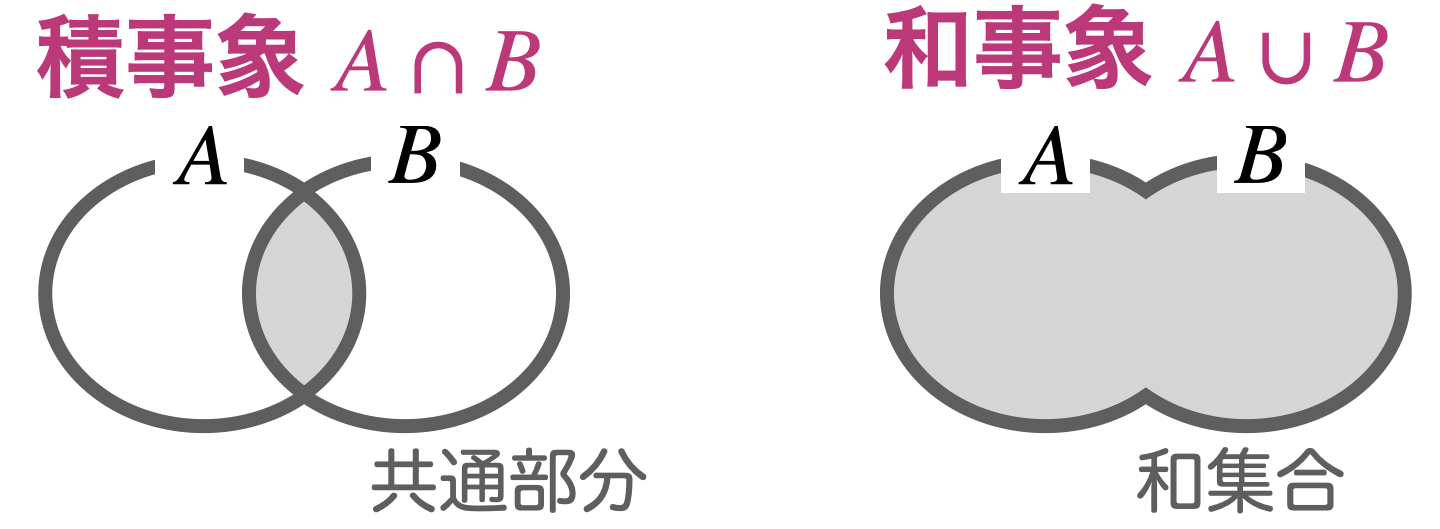
\includegraphics[width=10truecm]{./figure/f1-1.png}
\captionsetup{width=.9\linewidth}
\caption{%
  積事象 $A \cap B$ のベン図(左)と和事象 $A \cup B$ のベン図(右)。
}
\label{f:1.1}
\end{figure}

\begin{eg}[サイコロを1回投げる試行での積事象と和事象]
  サイコロを1回投げる。
  偶数の目が出るという事象を $A$、4以上の目が出るという事象を $B$ とすると、これらは
  \begin{align}
    A &= \{2,\, 4,\, 6 \}, \label{eq:1.3} \\
    B &= \{4,\, 5,\, 6 \} \label{eq:1.4}
  \end{align}
  という集合で表される。
  これらの積事象 $A \cap B$ と和事象 $A \cup B$ はそれぞれ、
  \begin{align}
    A \cap B &= \{4,\, 6 \}, \label{eq:1.5} \\
    B \cup B &= \{2,\, 4,\, 5,\, 6 \} \label{eq:1.6}
  \end{align}
  となる。
  ベン図を描いて確かめよ。
\end{eg}

\paragraph{排反事象}

サイコロを1回投げる試行について(再び)考えよう。
事象 $A$ :「偶数の目が出る」と事象 $B$ :「3の目が出る」の積事象 $A \cap B$ は、
\begin{align}
  A \cap B = \varnothing\, \text{(空事象)} \label{eq:1.7}
\end{align}
である(図\ref{f:1.2})。
つまり、事象 $A$ と事象 $B$ は同時には起こらない。
この時、事象 $A$ と事象 $B$ は\textbf{互いに排反}である、または、\textbf{互いに排反事象}であるという。

\begin{figure}[] 
\centering 
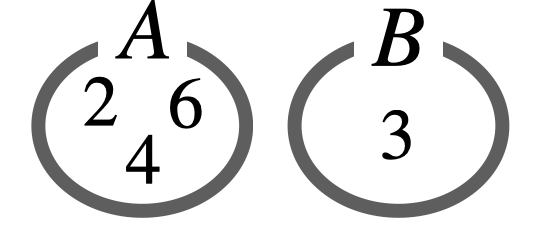
\includegraphics[width=6truecm]{./figure/f1-2.png}
\captionsetup{width=.9\linewidth}
\caption{%
  事象 $A = \{2,\, 4,\, 6\}$ と事象 $B = \{3\}$ のベン図。
  $A \cap B = \varnothing$ つまり、ベン図でこれらの集合は交わらない。
  3つ以上の事象についても、ベン図を描いて交わらないならば、それらは互いに排反である。
}
\label{f:1.2}
\end{figure}

\subsection{確率の計算と同様に確からしい根元事象について注意}

ついに確率の計算が始まる。

\paragraph{確率の計算}

ある1つの試行について、根元事象のどれが起こることも同じ程度に期待される時、これらの根元事象は\textbf{同様に確からしい}という。

全事象の\textbf{どの根元事象も同様に確からしいとき}、事象 $A$ の確率 $P(A)$ は
\begin{oframed}
  \begin{align}
    P(A) = \frac{\text{事象}\, A \text{の要素の個数}\, n(A)}{\text{全事象}\, U \text{の要素の個数}\, n(U)} \label{eq:1.8}
  \end{align}
\end{oframed}
\noindent
で計算される。

\begin{eg}[「どの根元事象も同様に確からしい」に注意せよ!] \label{eg:1.1}
  3枚のカードがあり、それぞれ0, 1, 2と書かれている。
  カードを裏返しにしてよくきり、1枚選ぶ。
  数字を確認したあと、そのカードは戻してよくシャッフルし、再び1枚選んで数字を確認する。
  選んだ2つのカードに書かれた数字の和が3となる確率はいくらか。

  \textbf{(答え?)}
  2つの数字の和の候補は $0,\, 1,\, 2,\, 3,\, 4$ だから、全事象は、
  \begin{align}
    \{0,\, 1,\, 2,\, 3,\, 4\} \label{eq:1.9}
  \end{align}
  である。
  したがって、
  \begin{align}
    \text{和が3となる確率} = \frac{\text{事象「和が3」の要素数}}{\text{全事象の要素数}} = \frac{1}{5} \label{eq:1.10}
  \end{align}
  となる。\mbox{}\\

  この解答は一見もっともらしいが、根本的な誤りがある。
  反省すべきは\eqref{eq:1.9} のように根元事象を
  \begin{align}
    \{0\},\,\{1\},\,\{2\},\,\{3\},\,\{4\} \label{eq:1.10.1}
  \end{align}
  としてしまった点である。
  確率の求め方\eqref{eq:1.8}を使えるのは、根元事象が同様に確からしい場合であった。
  \eqref{eq:1.10.1}は同様に確からしい根元事象ではない。
  なぜならば、(1枚目のカードの数字, 2枚目のカードの数字)と表すことにすると、
  \begin{center}
  \begin{tabular}{c|ccccc} \hline
    和 & 0 & 1 & 2 & 3 & 4 \\ \hline
    2枚の & (0, 0) & (0, 1) & (0, 2) & (1, 2) & (2, 2) \\
    組合せ &  & (1, 0) & (1, 1) & (2, 1) &  \\
     &  &  & (2, 0) & & \\ \hline
  \end{tabular}
  \end{center}
  のように0〜4の各和にカードの選ばれ方が対応しており、それぞれの場合の数が異なっているからだ。
  表の下側に現れた2枚の組合せ $(0,\, 0),\, (0,\, 1),\, \cdots ,\, (2,\,2)$ は、どれが起こることも同様に期待できる。
  よって、今考えている試行において根元事象として選ぶべきは、2つの数字の和ではなく、2枚のカードの組合せであった。

  \textbf{こっちが正しい(答え)}
  根元事象を2枚のカードの組合せとして、(上の表を見ながら)2つの数字の和が3となる確率を正しく計算すると、
  \begin{align}
    \text{和が3となる確率} = \frac{2}{9} \label{eq:1.10}
  \end{align}
  となる。
\end{eg}

くり返しになるが、確率の定義\eqref{eq:1.8}は、\textbf{全事象のどの根元事象も同様に確からしいときに限って使える}(やや不自由な)ものである。
つまり我々は確率を計算する際、まず、同様に確からしい根元事象を探さなければならない。
上の例では、
\begin{quotation}
  だめ:根元事象は $\{0\},\,\{1\},\,\{2\},\,\{3\},\,\{4\}$ だ!
  
  OK:根元事象は $\{(0,\, 0)\},\, \{(0,\, 1)\},\, \cdots ,\, \{(2,\,2)\}$ だ!
\end{quotation}
であった。

複数個のサイコロや複数個の硬貨などが登場する場合に、名前をつけてそれらを区別したり、(例\ref{eg:1.1}のような)同じ操作を繰り返し行う場合に「1回目」「2回目」・・・のように回数でそれらを区別したりするのが「同様に確からしい根元事象探し」の常套手段である。

\begin{eg}[複数個の硬貨に名前をつけて区別]
  2枚の硬貨を同時に投げる時、2枚とも表が出る確率を計算せよ。

  \textbf{(答え)}
  硬貨が2枚登場するので、1つを硬貨 A、もう1方を硬貨 B と名付けて区別する。
  (硬貨 A の表裏, 硬貨 B の表裏) と表すと、根元事象は
  \begin{align}
    \{(\text{表}, \text{表})\},\, \{(\text{表}, \text{裏})\},\, \{(\text{裏}, \text{表})\},\, \{(\text{裏}, \text{裏})\} \label{eq:1.11}
  \end{align}
  のように選べば、これらは同様に確からしい($\{\text{2枚とも表}\},\, \{\text{1枚は表、1枚は裏}\},\, \{\text{2枚とも裏}\},\,$ は同様に確からしいと言えない)。
  したがって、2枚とも表が出る確率は、
  \begin{align}
    P(\text{2枚とも表}) = \frac{1}{4} \label{eq:1.12}
  \end{align}
  である。
\end{eg}

\subsection{確率の基本性質}

\paragraph{確率の基本性質その1}

\ref{ss:1.1}節で述べたように、事象 $A$ は全事象 $U$ の部分集合で表すことができるので、$A$ の要素の個数 $n(A)$ について、
\begin{align}
  n(\varnothing) \leqq n(A) \leqq n(U) \label{eq:1.14}
\end{align}
が成り立つ。
各辺を $n(U)$ で割ると、
\begin{align}
  \frac{n(\varnothing)}{n(U)} \leqq \frac{n(A)}{n(U)} \leqq \frac{n(U)}{n(U)} \label{eq:1.16}
\end{align}
すなわち、
\begin{oframed}
\begin{align}
  0 \leqq P(A) \leqq 1 \label{eq:1.17}
\end{align}
\end{oframed}
\noindent
が成り立つことがわかる。
ただし、最左辺の変形には、空事象 $\varnothing$ は要素を持たない集合で表されるから、$n(\varnothing) = 0$ となることを利用した。
中辺の変形には確率の定義\eqref{eq:1.8}を使った。
\eqref{eq:1.16}と\eqref{eq:1.17}を見比べると、$P(A) = 0$ は $A = \varnothing$ の時に、$P(A) = 1$ は $A = U$ の時に成り立つことがわかる。

\paragraph{確率の基本性質その2(確率の加法定理)}

事象 $A$ と事象 $B$ は\textbf{互いに排反である} とする。
これらの和事象 $n(A \cup B)$ の要素の個数は、
\begin{align}
  n(A \cup B) = n(A) + n(B) \label{eq:1.18}
\end{align}
と書ける。
図\ref{f:1.2}からも明らかなように、2つの集合が交わらないので各集合の要素数を単純に足し合わせたものが和事象 $A \cup B$ の要素数になるのだ。

確率の定義\eqref{eq:1.8}と\eqref{eq:1.18}を用いることで、和事象 $A \cup B$ の確率 $P(A \cup B)$ は、
\begin{align}
  P(A \cup B) &= \frac{n(A \cup B)}{n(U)} \notag \\
              &= \frac{n(A) + n(B)}{n(U)} \notag \\
              &= \frac{n(A)}{n(U)} + \frac{n(B)}{n(U)} 
\end{align}
となるので、
\begin{oframed}
  \begin{align}
    P(A \cup B) &= P(A) + P(B) \label{eq:1.19}
  \end{align}
\end{oframed}
\noindent
という表式が得られる。
\eqref{eq:1.19} は\textbf{確率の加法定理} と呼ばれる。

\eqref{eq:1.19} は、事象 $A$ と事象 $B$ が互いに排反であるときに限って使えるということに注意せよ。
$A$ と $B$ が互いに排反でない場合への拡張は次節でおこなう。

\begin{eg}[確率の加法定理の問題]
  2つのサイコロを同時に投げる時、出た目の和が5の倍数になる確率を計算せよ。

  \textbf{(答え)}
  2つの目の和としてとり得るのは、2〜12の整数である。
  この内、5の倍数は5と10であるから、事象 $A$「出た目の和が5になる」と事象 $B$ 「出た目の和が10になる」という2つの排反な事象の確率をそれぞれ計算し、最後に足し合わせればよい。
  (1つ目のサイコロの目, 2つ目のサイコロの目)のように表すことにすれば、$A = \{(1, 4),\, (2, 3),\, (3, 2),\, (4, 1)\},\, B = \{(4, 6),\, (5, 5),\, (6, 4)\}$ なので、確率の定義\eqref{eq:1.8}より、
  \begin{align}
    P(A) &= \frac{n(A)}{n(U)} = \frac{4}{36}, \\
    P(B) &= \frac{n(B)}{n(U)} = \frac{3}{36}
  \end{align}
  と求められる。
  確率の加法定理\eqref{eq:1.18}より、
  \begin{align}
    P(A \cup B) = P(A) + P(B) = \frac{4}{36} + \frac{3}{36} = \frac{7}{36}
  \end{align}
  となる。
\end{eg}

\section{様々な確率の計算}

\subsection{和事象と余事象の確率}

\paragraph{和事象の確率}

前節で強調したように、確率の加法定理\eqref{eq:1.19}は互いに排反な事象の和事象を計算するものであった。
ここでは、互いに排反とは限らない事象についても和事象を計算することが目標である。

互いに排反ではない2つの事象 $A,\, B$ について、これらの和事象の要素の個数は
\begin{align}
  n(A \cup B) = n(A) + n(B) - n(A \cap B) \label{eq:2.1}
\end{align}
と表される(図\ref{f:2.1}を参照、もしくは教科書やノートの集合のページを復習せよ)。
確率の定義\eqref{eq:1.8}とあわせて、
\begin{align}
  P(A \cup B) &= \frac{n(A \cup B)}{n(U)} \notag \\
              &= \frac{n(A) + n(B) - n(A \cap B)}{n(U)} \notag \\
              &= \frac{n(A)}{n(U)} + \frac{n(B)}{n(U)} - \frac{n(A \cap B)}{n(U)}
\end{align}
であるから、和事象の確率の公式
\begin{oframed}
  \begin{align}
    P(A \cup B) &= P(A) + P(B) - P(A \cap B) \label{eq:2.2}
  \end{align}
\end{oframed}
\noindent
が導かれる。

\begin{figure}[] 
\centering 
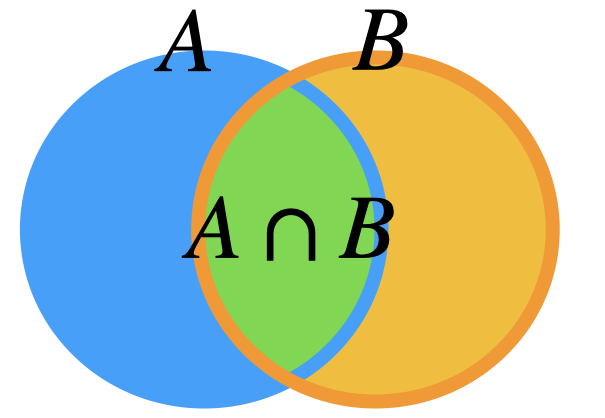
\includegraphics[width=6truecm]{./figure/f2-1.png}
\captionsetup{width=.9\linewidth}
\caption{%
  互いに排反でない事象 $A$ と事象 $B$ のベン図。
  和事象 $A \cup B$ の要素の個数はどう表されるか。
  各集合の要素の個数を $n(A) + n(B)$ のように足し算してしまうと、共通部分 $A \cap B$ (図の緑色の部分)を余分に数え上げることになる。
  したがって、2つの集合の要素数の和 $n(A) + n(B)$ から、重複して数えてしまった $n(A \cap B)$ を引いたものが、和事象 $A \cup B$ の要素の個数となる:$n(A \cup B) = n(A) + n(B) - n(A \cap B)$.
}
\label{f:2.1}
\end{figure}

事象 $A$ と事象 $B$ が互いに排反(図\ref{f:1.2}のように、ベン図で描けば互いに交わらない)であれば、$A \cap B = \varnothing$ つまり $ n(A \cap B) = 0$ だから、$P(A \cap B) = \dfrac{n(A \cap B)}{n(U)} = 0$ となるので、\eqref{eq:2.2}の右辺第3項が消えて、
\begin{align}
  P(A \cup B) = P(A) + P(B) \label{eq:2.3}
\end{align}
が得られる。
この表式は、\pageref{eq:1.19}ページで紹介した確率の加法定理\eqref{eq:1.18}である。
つまり、確率の加法定理は$A \cap B = \varnothing$($A$ と $B$ は互いに排反事象)という特殊な場合として、和事象の確率の公式\eqref{eq:2.2}に含まれている。

\begin{eg}[倍数と確率]
  1から100までの数字が書かれた100枚のカードがある。
  カードをよくシャッフルして1枚取り出す時、その番号が4の倍数または6の倍数である確率を計算せよ。

  \textbf{(答え)}
  取り出したカードの数字が4の倍数である事象を $A$、6の倍数である事象を $B$ とする。
  ここで、$A \cup B$ は4の倍数であり6の倍数でもある(つまり12の倍数)カードを引くという事象である。
  各事象の要素の個数は $n(A) = 25,\, n(B) = 16,\, n(A \cup B) = 8$ であるから、各事象の確率は、
  \begin{align}
    P(A) = \frac{25}{100},\, P(B) = \frac{16}{100},\, P(A \cup B) = \frac{8}{100} \label{eq:2.3.1}
  \end{align}
  と計算できる。
  もちろん $n(U) = 100$ と確率の定義 \eqref{eq:1.8} を使った。
  和事象の確率の公式\eqref{eq:2.2}より、
  \begin{align}
    P(A \cup B) &= P(A) + P(B) - P(A \cap B) \notag \\
                &= \frac{25}{100} + \frac{16}{100} - \frac{8}{100} = \frac{33}{100} \label{eq:2.3.2}
  \end{align}
  が得られる。
\end{eg}

\paragraph{余事象の確率}

事象 $A$ に対して、$A$ が起こらないという事象を\textbf{余事象}といい、補集合 $\overline{A}$ で表す。
図\ref{f:2.2}を見ると明らかなように、
\begin{align}
  n(\overline{A}) = n(U) - n(A) \label{eq:2.4}
\end{align}
という関係が成り立つ。
これまでと同様に、$n(\cdot)$ は各集合の要素の個数を表す。
確率の定義\eqref{eq:1.8}に\eqref{eq:2.4}を適用すれば、
\begin{align}
  P(\overline{A}) &= \frac{n(\overline{A})}{n(U)} \notag \\
                  &= \frac{n(U) - n(A)}{n(U)} \label{eq:2.5}
\end{align}
となるので、余事象の確率の公式
\begin{oframed}
  \begin{align}
     P(\overline{A}) = 1 - P(A) \label{eq:2.6}
  \end{align}
\end{oframed}
\noindent
が導かれる。
もちろん、\eqref{eq:2.6}の $P(\overline{A})$ と $P(A)$ を移行すれば\footnote{%
  \eqref{eq:2.6} の $A$ を $\overline{A}$ に置き換えて、補集合の性質 $\overline{\overline{A}} = A$ を利用しても、\eqref{eq:2.7}を得られる。
}
、
\begin{align}
  P(A) = 1 - P(\overline{A}) \label{eq:2.7}
\end{align}
という表式も得られる。


\begin{figure}[] 
\centering 
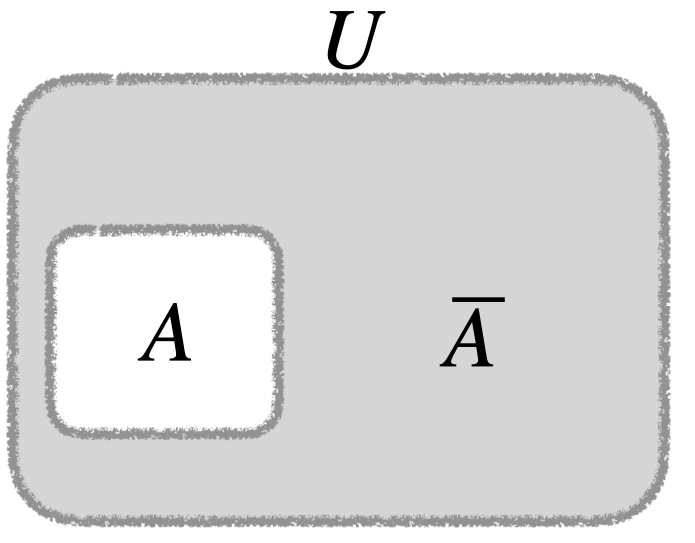
\includegraphics[width=6truecm]{./figure/f2-2.png}
\captionsetup{width=.9\linewidth}
\caption{%
  事象 $A$ とその余事象 $\overline{A}$ のベン図。
}
\label{f:2.2}
\end{figure}

\begin{eg}[ド・メレの問題]
  次のどちらの賭けの勝率が高いか。
  \begin{enumerate}
  \item サイコロを4回投げて、1回でも6の目が出たら勝ち。
  \item サイコロ2つを同時に24回投げて、1回でもゾロ目 (6, 6) が出たら勝ち。
  \end{enumerate}

  \textbf{(答え)}
  \begin{enumerate}
  \item 求めたいのは、事象 $A$ 「4回中少なくとも1回は6の目が出る」の確率 $P(A)$ である。
    $A$ の余事象 $\overline{A}$ は「4回全て1以外の目が出る」であり、この確率 $P(\overline{A})$ は
    \begin{align}
      P(\overline{A}) = \frac{n(\overline{A})}{n(U)} = \frac{5 \times 5 \times 5 \times 5}{6 \times 6 \times 6 \times 6} = \left( \frac{5}{6} \right)^4 \label{eq:2.7.1}
    \end{align}
    と求まる。
    余事象の確率の公式\eqref{eq:2.7}より、
    \begin{align}
      P(A) = 1 - \left( \frac{5}{6} \right)^4 \label{eq:2.7.2}
    \end{align}
    とわかる。
  \item 求めたいのは、事象 $B$ 「24回中少なくとも1回は (6, 6) が出る」の確率 $P(B)$ である。
    $B$ の余事象 $\overline{B}$ は「24回全て(6, 6)以外の目が出る」であり、この確率 $P(\overline{B})$ は
    \begin{align}
      P(\overline{B}) = \frac{n(\overline{B})}{n(U)} = \frac{35^{24}}{36^{24}} = \left( \frac{35}{36} \right)^{24} \label{eq:2.7.3}
    \end{align}
    となる。
    余事象の確率の公式\eqref{eq:2.7}を用いれば、
    \begin{align}
      P(B) = 1 - \left( \frac{35}{36} \right)^{24} \label{eq:2.7.4}
    \end{align}
    となる。
  \end{enumerate}

  計算機の助けを借りると、$P(A) = 0.518,\, P(B) = 0.491$ が得られる。
  よって、1つめ賭けの方が勝率が高い。
\end{eg}

\subsection{独立な試行の確率}

\paragraph{独立な試行とは}

2つの試行について、互いに他方の結果に影響を及ぼさない時、これらの試行は\textbf{独立}であるという。
硬貨を何回か続けて投げる時、表のあとは裏が出やすいということはない。
つまり、毎回のコイントスは独立である。

\begin{eg}[引いたカードを戻すか戻さないかで独立かどうか変わる]
  袋に赤玉が3つと白玉が2つは入っている。
  目隠しをして袋から玉を一つ取り出す。
  玉の色を確認したのちに、

  \textbf{(a)~玉を戻さずに}
  もう一度玉を取り出す。
  1回目と2回目で袋の中の玉の状態が変わってしまうので、これらは独立な試行ではない。

  \textbf{(b)~玉を戻してから}
  もう一度玉を取り出す。
  1回目と2回目で袋の中の玉の状態は同じ。
  よって、1回目で何色を取り出そうが2回目の結果には影響を及ぼさない。
  これらは独立な試行となる。
\end{eg}

\paragraph{独立な試行の計算}

次の例題の考察から、独立な試行の確率の公式を導こう(公式と呼ぶは大袈裟な気もするが)。

\begin{eg}[独立な試行の確率の公式を導く]
  a, b, c の3種類のアルファベットが印字されたカードと、1, 2, 3, 4がそれぞれ印字された数字カードがある。
  3枚のアルファベットカードから1枚、4枚の数字カードのから1枚を(目隠しをして)選ぶ。
  これらは独立な試行である。
  この時、事象 $A$「アルファベットカードはbを引き、数字カードは1か3を引く」の確率 $P(A)$ を求めよ。

  \textbf{(答え)}
  $P(A) = n(A) /n(U)$ のように事象 $A$ の確率を求められるので、図\ref{f:2.3}を見ながら $n(A)$ と $n(U)$ を数えれば、
  \begin{align}
    n(A) &= 1 \times 2,\,  n(U) = 3 \times 4 \label{eq:2.8}
  \end{align}
  となる。
  よって、
  \begin{align}
    P(A) &= \frac{n(A)}{n(U)} = \frac{1 \times 2}{3 \times 4} \notag
  \end{align}
  であるが、最右辺をよく見ると、
  \begin{align}
    &= \frac{1}{3} \times \frac{2}{4} \notag \\
    &= P(\text{アルファベットカードのbを引く}) \times P(\text{数字カードの2または4を引く}) \label{eq:2.9}
  \end{align}
  という形をしていることに気づく。
  つまり、アルファベットカードから1枚選ぶという試行においてbを選ぶ確率と数字カードから1枚選ぶという試行において1または3を選ぶ確率を別個計算しておき、それらをかけ合わせたものが $P(A)$ となる。
  
  \begin{figure}[] 
    \centering 
    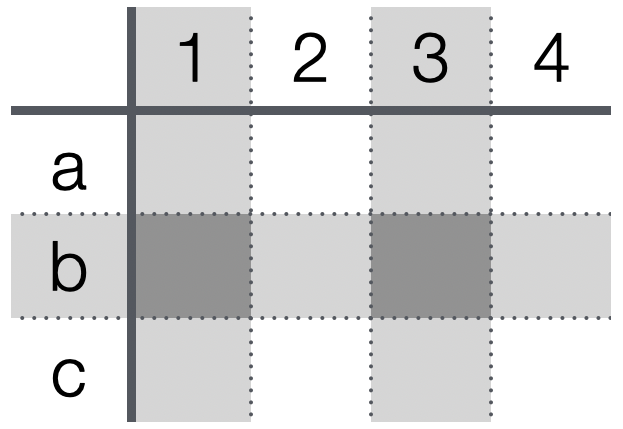
\includegraphics[width=6truecm]{./figure/f2-3.png}
    \captionsetup{width=.9\linewidth}
    \caption{%
      3枚のアルファベットカードから1枚選ぶ試行と4枚の数字カードから1枚ずつ選ぶ試行において、起こりうる結果をまとめたもの。
      選ばれるカードの組合せの総数(つまり全事象 $U$ の要素の個数)は表のマス目の個数であるから $n(U) = 3 \times 4$ となる。
      アルファベットカードからbを引き、数字カードから1または3を引くという事象 $A$ は、表の濃く塗りつぶしてあるマスに対応しており、$n(A) = 1 \times 2$ である。
    }
    \label{f:2.3}
  \end{figure}
\end{eg}

この例でわかった事実をほんのちょっとだけ一般的に書き表そう:
独立な試行 $\mathrm{T}_1,\, \mathrm{T}_2$ について、試行 $\mathrm{T}_1$ では事象 $A$ が起こり、試行 $\mathrm{T}_2$ では事象 $B$ が起こるという事象が起こる確率 $P$ は、
\begin{oframed}
  \begin{align}
     P = P(A)P(B) \label{eq:2.10}
  \end{align}
\end{oframed}
\noindent
で計算される。

\begin{eg}[俺にはKISUKEしかない]
  KISUKE には4つのステージがある:
  \begin{enumerate}
  \item 5杯のジュースのうち、1杯は超酸っぱい!ラッピージュース。
  \item 4つのジャンプ台のうち、1つは着地地点に足つぼマット。
  \item 3つのシュークリームのうち、1つは激辛からし入り。
  \item 2脚の椅子のうち、1脚はビリビリ椅子。
  \end{enumerate}
  ダメージをくらったらそこで失格。
  KISUKE をクリアする確率を計算せよ。

  \textbf{(答え)}
  1st ステージから 4th ステージまで、それぞれの挑戦は独立である。
  だから、各ステージでの成功確率を計算し、最後にそれらをかけ算すればよい:
  \begin{align}
    P &= \frac{4}{5} \times \frac{3}{4} \times \frac{2}{3} \times \frac{1}{2} =\frac{1}{5}.
  \end{align}
\end{eg}

\subsection{反復試行の確率}

独立な試行を繰り返すという試行を\textbf{反復試行}という。

\begin{eg}[サイコロを使った反復試行]
  サイコロを4回投げる。
  4回の試行はお互いの結果に影響を及ぼさない。
  例えば、1が出た後は1が出づらいということはない。
  つまりこれらは独立な試行であり、独立な試行を繰り返しておこなっているので反復試行と言える。
  4回中ちょうど2回、1の目が出る確率を計算せよ。

  \textbf{(答え)}
  まず、4回中2回、1の目が出るシチュエーションを全て列挙しよう:
  
    \begin{center}
      \begin{tabular}{ccccc} \hline
        & 1回目 & 2回目 & 3回目 & 4回目 \\ \hline
        $A$ & {\color{red} 1} & {\color{red} 1} & 1以外 & 1以外 \\
        $B$ & {\color{red} 1} & 1以外 & {\color{red} 1} & 1以外 \\
        $C$ & {\color{red} 1} & 1以外 & 1以外 & {\color{red} 1} \\
        $D$ & 1以外 & {\color{red} 1} & {\color{red} 1} & 1以外 \\
        $E$ & 1以外 & {\color{red} 1} & 1以外 & {\color{red} 1} \\
        $F$ & 1以外 & 1以外 & {\color{red} 1} & {\color{red} 1} \\ \hline
      \end{tabular}
    \end{center}

    表から全6パターンあることがわかる。
    総数の``6''は、4回の試行に対し2つの{\color{red}1}を割り当てる場合の数の計算であるから、${}_4 \mathrm{C}_2$ で求められる。
    説明の都合で6つそれぞれに $A$〜$F$ と名前をつけた。
    $A$ が起こる確率は、独立な試行の確率の公式\eqref{eq:2.10}より、
    \begin{align}
      P(A) = \frac{1}{6} \times \frac{1}{6} \times \frac{5}{6} \times \frac{5}{6} = \left( \frac{1}{6} \right)^2 \times \left( \frac{5}{6} \right)^2
    \end{align}
    である。
    $B,\,C,\, \cdots ,\, F$ が起こる確率も同様に、
    \begin{align}
      P(B) &= \frac{1}{6} \times \frac{5}{6} \times \frac{1}{6} \times \frac{5}{6} = \left( \frac{1}{6} \right)^2 \times \left( \frac{5}{6} \right)^2, \\
      P(C) &= \frac{1}{6} \times \frac{5}{6} \times \frac{5}{6} \times \frac{1}{6} = \left( \frac{1}{6} \right)^2 \times \left( \frac{5}{6} \right)^2, \\
      P(D) &= \frac{5}{6} \times \frac{1}{6} \times \frac{1}{6} \times \frac{5}{6} = \left( \frac{1}{6} \right)^2 \times \left( \frac{5}{6} \right)^2, \\
      P(E) &= \frac{5}{6} \times \frac{1}{6} \times \frac{5}{6} \times \frac{1}{6} = \left( \frac{1}{6} \right)^2 \times \left( \frac{5}{6} \right)^2, \\
      P(F) &= \frac{5}{6} \times \frac{5}{6} \times \frac{1}{6} \times \frac{1}{6} = \left( \frac{1}{6} \right)^2 \times \left( \frac{5}{6} \right)^2
    \end{align}
    と計算される。
    結局、$(1/6)^2 \times (5/6)^2$ が、${}_4 \mathrm{C}_2 = 6$ 組できるとわかる。
    
    $A,\, \cdots,\, F$ は互いに排反であるから(排反な事象については\ref{ss:1.1}節を復習せよ)、確率の加法定理\eqref{eq:1.19}が利用できる。
    ゆえに、4回中ちょうど2回、1の目が出る確率 $P$ は、
    \begin{align}
      P =& P(A) + P(B) + P(C) + P(D) + P(E) + P(F) \notag \\
      =& \left( \frac{1}{6} \right)^2 \times \left( \frac{5}{6} \right)^2 + \left( \frac{1}{6} \right)^2 \times \left( \frac{5}{6} \right)^2 + \left( \frac{1}{6} \right)^2 \times \left( \frac{5}{6} \right)^2 \notag \\
         &+ \left( \frac{1}{6} \right)^2 \times \left( \frac{5}{6} \right)^2 + \left( \frac{1}{6} \right)^2 \times \left( \frac{5}{6} \right)^2 + \left( \frac{1}{6} \right)^2 \times \left( \frac{5}{6} \right)^2 \notag \\
        =& {}_4 \mathrm{C}_2 \times \left( \frac{1}{6} \right)^2 \times \left( \frac{5}{6} \right)^2 \label{eq:2.11}
    \end{align}
    で求められる。    
\end{eg}

一般に、ある試行を $n$ 回繰り返す時、事象 $A$ がちょうど $r$ 回起こる確率 $P$ は、
\begin{oframed}
  \begin{align}
     P = {}_n \mathrm{C}_r \times \left( P(A) \right)^r \times \left( 1 - P(A) \right)^{n-r}  \label{eq:2.12}
  \end{align}
\end{oframed}
\noindent
である。
上のサイコロの例を思いだせば、すぐに\eqref{eq:2.12}は復元できるだろう。
だから無理に公式として覚えるまでもない。
もちろん、\eqref{eq:2.12}において、$n = 4,\, r = 2,\, P(A) = 1/6$ と置き換えれば\eqref{eq:2.11}が導かれる。

\section{条件付き確率}

\subsection{条件付き確率} \label{ss:3.1}

\paragraph{条件付き確率ってなんなのさ}

生徒会が全校生徒100人にアンケートをとった。
アンケートは「あなたは文系ですか、理系ですか?」と「あなたは爬虫類を飼っていますか?」の2問。
結果は表\ref{t:3.1}のようになった。

\begin{table}[tb]
\captionsetup{width=.9\linewidth}
\caption{%
  生徒100人に「文系か理系か」、「爬虫類を飼っているか」という質問をして得られたデータ。
  100人からランダムに1人選んだとき、その生徒が文系であるという事象 $A$、理系であるという事象 $\overline{A}$、爬虫類を飼っているという事象 $B$、爬虫類を飼っていないという事象 $\overline{B}$ の確率を考える。
  単に選ばれた生徒が文系である確率を計算したければ、表の4行目に着目することで、 $P(A) = 65/100$ が求まる。
  選ばれた生徒が爬虫類を飼っていることをあらかじめ知らされている場合、表の2行目に着目し、条件付き確率 $P_B (A) = 10/25$ が求まる。
  同じ「文系である確率」の計算でも、爬虫類を飼っているかどうかの情報の有無によって確率の計算過程(ここでは表のどこに注目して計算を進めるか)が変わる。
}
\label{t:3.1}
\centering
\begin{tabular}{c|cc|c} \hline
 & 文系 $A$ & 理系 $\overline{A}$ & 計 \\ \hline
爬虫類を飼っている $B$ & 10 & 15 & 25 \\
爬虫類を飼っていない $\overline{B}$ & 55 & 20 & 75 \\ \hline
計 & 65 & 35 & 100 \\ \hline
\end{tabular}    
\end{table}

アンケートに答えた100人の中からランダムに1人選び出したとき、その生徒が文系であるという事象を $A$、その生徒が爬虫類を飼っているという事象を $B$ とする。
すると、その生徒が理系である事象と爬虫類の飼い主ではないという事象はそれぞれ $A$, $B$ の余事象 $\overline{A}$, $\overline{B}$ で表される。

表\ref{t:3.1}から、回答者100人のうち文系は65人いるとわかった。
この事実をもとに、事象 $A$ の確率(選ばれたその生徒が文系である確率)は、
\begin{align}
  P(A) = \frac{65}{100} = \frac{13}{20} \label{eq:3.1}
\end{align}
と計算できる。
再び100人の中から1人をランダムに選ぶ。
今回はあらかじめその生徒が爬虫類を飼っていることがわかっていたとする。
表\ref{t:3.1}から、爬虫類を飼っている生徒は25人いて、そのうち文系は10人いると読み取れるので、この生徒が文系である確率は、
\begin{align}
  P(A) = \frac{10}{25} = \frac{2}{5} \label{eq:3.2}
\end{align}
となる。

(\ref{eq:3.1})も(\ref{eq:3.2})も文系である確率 $P(A)$ を計算するものだが、値が異なっている。
なぜだろうか。
(\ref{eq:3.2})を計算する際、事前に「その生徒が爬虫類を飼っている(事象 $B$)」という情報を得ていた。
言い換えると、事象 $B$ が起こったことがわかった上で事象 $A$ の確率を計算していた。
一方で、(\ref{eq:3.1})のときは爬虫類を飼っているかの情報はなかった。
事前情報の有無によって確率の計算結果が変わってしまうのだ(表\ref{t:3.1}の説明も参照)。
(\ref{eq:3.2})について、事象 $A$ の確率を計算する際に「事象 $B$ が起こったことを事前に知っていましたよ」ということを強調するために、確率の記号として $P(A)$ に下付き文字を加えた $P_B (A)$ を用いる。
$P_B (A)$ を事象 $B$ が起こったときに事象 $A$ が起こる\textbf{条件付き確率}と呼ぶ。

\paragraph{条件付き確率の計算}

条件付き確率(\ref{eq:3.2})を見ると、文系かつ爬虫類を飼っている生徒の人数 $n(A \cap B) = 10\,$人を、爬虫類を飼っている生徒の人数 $n(B) = 25\,$ 人で割っているとわかる。
つまり、
\begin{oframed}
  \begin{align}
    P_B (A) = \frac{n(A \cap B)}{n(B)} \label{eq:3.3}
  \end{align}
\end{oframed}
\noindent
と書ける。
この式の右辺の分母分子を $n(U)$ で割ると、
\begin{oframed}
  \begin{align}
    P_B (A) = \frac{P(A \cap B)}{P(B)} \label{eq:3.4}
  \end{align}
\end{oframed}
\noindent
という表式も得られる。
我々は、(\ref{eq:3.3})や(\ref{eq:3.4})を用いて、事象 $B$ が起こったときに事象 $A$ が起こる条件付き確率 $P_B (A)$ を求める。

\begin{eg}[条件付き確率の計算問題]
  表 \ref{t:3.1}の100人から選び出された生徒が理系であることがわかっているとき、その生徒が爬虫類を飼っている確率 $P_{\overline{A}} (B)$ を計算せよ。

  \textbf{(答え)}
  (\ref{eq:3.3})より、
  \begin{align}
    P_{\overline{A}} (B) = \frac{n(\overline{A} \cap B)}{n(\overline{A})} = \frac{3}{7} \label{eq:3.5}
  \end{align}
  となる。
\end{eg}

\subsection{確率の乗法定理}

(\ref{eq:3.4})の両辺を $P(A)$ 倍すると、
\begin{oframed}
  \begin{align}
    P(A \cap B) = P(B) P_B (A) \label{eq:3.6}
  \end{align}
\end{oframed}
\noindent
が得られる。
これは、\textbf{確率の乗法定理}と呼ばれる。

\begin{eg}[確率の乗法定理(\ref{eq:3.6})の使いどころ]
  箱に赤玉3個と白玉2個が入っている。
  目をつぶって箱から玉をひとつ取り出し、その玉を箱に戻さずにもう一度目をつぶって箱から玉を取り出した。
  2つとも赤玉である確率を計算せよ。

  \textbf{(答え)}
  1回目が赤玉である確率は$P(\text{1回目赤}) = 3/5$ で、1回目に赤玉を引いた時に2回目に赤玉を引く条件付き確率は$P_{\text{1回目赤}}(\text{2回目赤}) = 1/2$ となる。
  確率の乗法定理(\ref{eq:3.6})より、1回目も2回目も赤玉を取り出す確率は、
  \begin{align}
    P(\text{1回目赤} \cap \text{2回目赤})
    &= P(\text{1回目赤}) \times P_{\text{1回目赤}}(\text{2回目赤}) \notag \\
    &= \frac{3}{5} \times \frac{1}{2} \notag \\
    &= \frac{3}{10} \label{eq:3.7}
  \end{align}
  と計算される。
\end{eg}

\subsection{原因の確率}

\paragraph{本節でやりたいこと}

前節までに述べたことの繰り返しになるが、ある事象 $B$ が起こった時に事象 $A$ が起こる条件付き確率は $P_B (A)$ と表され、\eqref{eq:3.3}や\eqref{eq:3.4}で計算される。
あらかじめ知っている「$A$ が起こったという事実」をもとに、$B$ が起こる確率を計算している。

本節では、「『$A$が起こったという事実』を確認していないが、結果的に事象 $B$ が起こった。じゃあ $A$ が起こっていたのだろうか?」ということを確率を用いて考えたい。

\begin{eg}[spam メールの判別] \label{eg:3.3}
  受信者の意図を無視した一方的なメールをspamメールといい、spamではないものをhamと呼ぶ。

  手元に10000件のメールがあり、そのうち3000件がspamで残り7000件がhamである。
  spamメールのうち80%には本文に"claim"という単語が含まれている。
  一方、hamの5%には本文に"claim"という単語が含まれている。
  一応表にしておく:

  \begin{center}
  \begin{tabular}{c|cc|c} \hline
    & spam  ($A$) & ham ($\overline{A}$) & 計 \\ \hline
    claim が含まれる ($B$) & 2400 & 350 & 2750 \\
    claim が含まれない ($\overline{B}$) & 600 & 6650 & 7250 \\ \hline
    計 & 3000 & 7000 & 1000 \\ \hline
  \end{tabular}
  \end{center}

  この10000件のメールの中から、無作為に1件メールを選んだところ本文に"claim"という単語が含まれていた。
  このメールがspamである確率を計算せよ。

  \textbf{(答え)}
  選んだメールがspamであるという事象を $A$、選んだメールにclaimという単語が含まれている事象を $B$ とする。
  条件付き確率の公式\eqref{eq:3.3}より、
  \begin{align}
    P_B (A) = \frac{n(A \cap B)}{n(B)} = \frac{48}{55} \label{eq:3.8}
  \end{align}
  である。
  $n(\cdot)$ には表を睨みながら数字を代入するだけ。
  終わり!
  
  以上のように、表を書けば計算は一発だが、ここではあえて愚直に計算を進めよう。
  問題文に「10000件のメールがあり、そのうち3000件がspamで残り7000件がham」とあるので、
  \begin{align} 
    P(A) = \frac{3000}{10000},\, P(\overline{A}) = \frac{7000}{10000} \label{eq:3.9}
  \end{align}
  とわかる。
  同じく、「spamメールのうち80%には本文に"claim"という単語が含まれている。一方、hamの5%には本文に"claim"という単語が含まれている。」という文から、
  \begin{align} 
    P_A (B) = \frac{80}{100},\, P_{\overline{A}} (B) = \frac{5}{100} \label{eq:3.10}
  \end{align}
  もわかる。
  問題文から直ちに得られる\eqref{eq:3.9}, \eqref{eq:3.10} から $P_B (A)$ の表式を導くことが、ここでの目標である。

  我々の目的地である $P_B (A)$ は、条件付き確率の公式\eqref{eq:3.4}より、
  \begin{align}
    P_B (A) = \frac{P(A \cap B)}{P(B)} \label{eq:3.11}
  \end{align}
  と表された。
  この式の右辺の分子は確率の乗法定理\eqref{eq:3.6}より、
  \begin{align}
    P(A \cap B) = P(A) P_A (B) \label{eq:3.12}
  \end{align}
  と書ける。
  \eqref{eq:3.11}の右辺分母は、
  \begin{align}
    P(A) &= P(A \cap B) + P(A \cap \overline{B}) \notag \\
         &= P(A) P_A (B) + P(\overline{A}) P_{\overline{A}} (B) \label{eq:3.13}
  \end{align}
  と(かなりテクニカルに)変形できる。
  1行目では、$A = A \cap U = A \cap (B \cup \overline{B}) = (A \cap B) \cup (A \cap B)$ という(一見複雑そうに見える)変形をおこなったが、ベン図を描くのと直感的に意味を理解できる(図\ref{f:3.1})。
  2行目を導くために確率の乗法定理\eqref{eq:3.6}を利用した。
  \eqref{eq:3.12}と\eqref{eq:3.13}を\eqref{eq:3.11}に代入すれば、
  \begin{align}
    P_B (A) = \frac{P(A) P_A (B)}{P(A) P_A (B) + P(\overline{A}) P_{\overline{A}} (B)} \label{eq:3.14}
  \end{align}
  が得られる。
  右辺は、問題文からすぐに計算できる \eqref{eq:3.9}, \eqref{eq:3.10} だけで構成されている。
  先ほど提示した我々の目標が達成された!
  \eqref{eq:3.14} を「事象 $B$ が起こったことを知って、それが原因 $A$ から起こったと考えられる『原因の確率』」の公式だと認めしまい、\eqref{eq:3.9}や\eqref{eq:3.10}の計算結果を代入すれば、機械的に原因の確率は計算できる(実際にやってみよ)。
  ただし、今回の問題では表を書けば秒殺であった。

  \begin{figure}[] 
    \centering 
    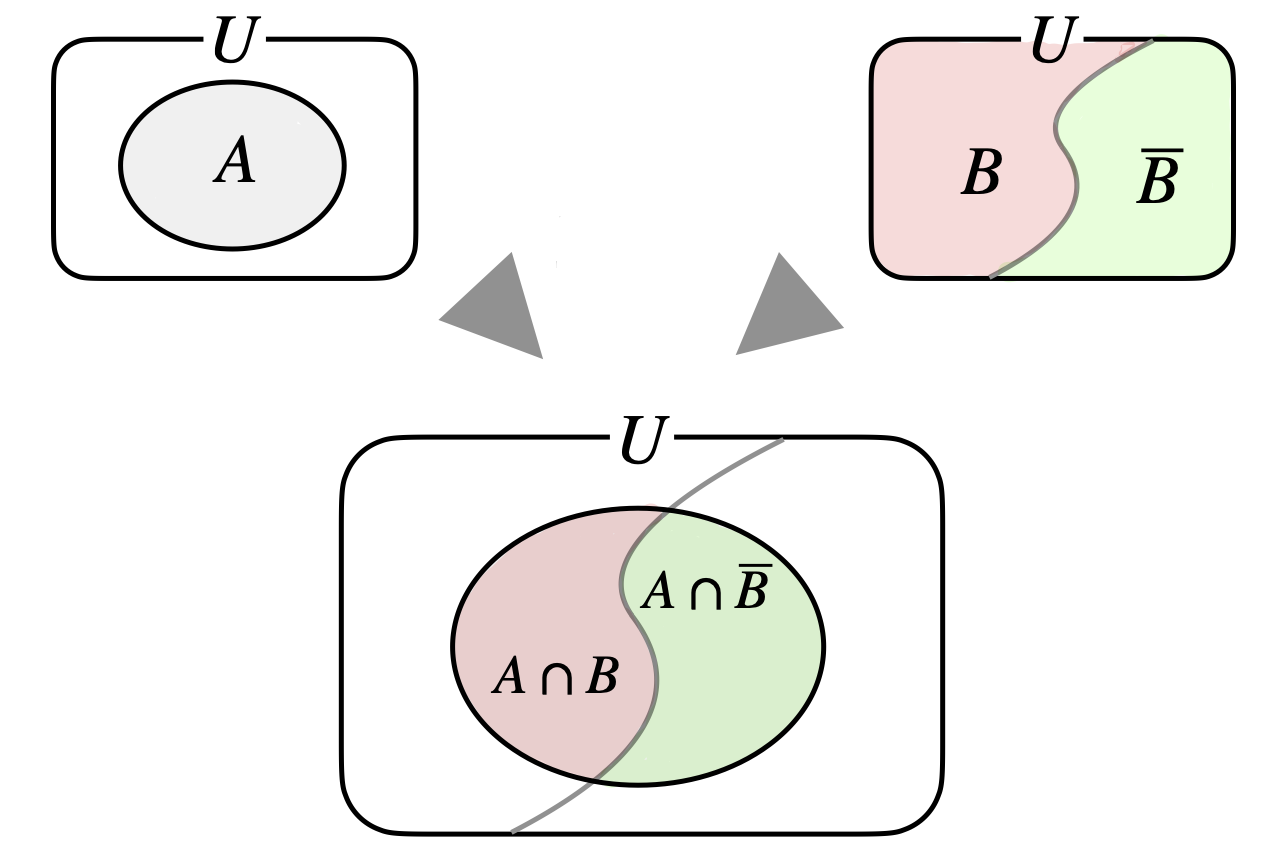
\includegraphics[width=10truecm]{./figure/f3-1.png}
    \captionsetup{width=.9\linewidth}
    \caption{%
      左上の図は全事象 $U$ と事象 $A$ のベン図。
      右上の図は全事象 $U$ と事象 $B$ とその余事象 $\overline{B}$ のベン図。
      これらを重ね合わせたものが下の図である。
      ここに示されているように、$A$ は $A \cap B$ と $A \cap \overline{B}$ の2つに分断できる。
      したがって、$n(A) = n(A \cap B) + n(A \cap \overline{B})$ であり、\eqref{eq:3.13}の1行目の変形:$P(A) = \dfrac{n(A)}{n(U)} = \dfrac{n(A \cap B) + n(A \cap \overline{B})}{n(U)} = P(A \cap B) + P(A \cap \overline{B})$ が導かれる。
    }
    \label{f:3.1}
  \end{figure}

  答えが長くなってしまったので、ここまでのストーリーをまとめておく。
  迷子になってしまった人はこれをロードマップに読み返してほしい。
  \begin{enumerate}
  \item 我々がはじめに与えられていた情報は $P(A),\, P(\overline{A}),\, P_A (B),\, P_{\overline{A}} (B)$ の4つの確率である(\eqref{eq:3.9}, \eqref{eq:3.10})。
  \item これらの確率を利用して $P_B (A)$ を計算したい。
  \item 条件付き確率の公式\eqref{eq:3.4}や確率の乗法定理\eqref{eq:3.6}を利用して $P_B (A) = \dfrac{P(A) P_A (B)}{P(A) P_A (B) + P(\overline{A}) P_{\overline{A}} (B)}$ が導けた!
  \end{enumerate}
\end{eg}

\begin{eg}[おまけの問題]
  ジョーカーを除いたトランプ52枚をよくシャッフルした後、伏せて机に置く。
  その束から無作為に1枚選んで\textbf{表を開けずに}適当な箱に封印する。
  残りの束から無作為に1枚引いて表を見たところ、ハートのAであった。
  このとき、はじめに引いて封印していたカードが赤か黒かで賭けをしたい。
  \begin{description}
  \item[和さん]  「2枚目のカードが赤だったから、1枚目にはきっと黒のカードを引いただろう。」
  \item[健さん]  「1枚目を引く段階では、黒と赤が半々なのでどちらを引く確率は$1/2$である。
    それを封印した後はその箱に手を加えていないのだから、確率は$1/2$のまま変わるわけがない。
    したがって、赤と黒のどっちを選んでも確率は同じである。」
  \end{description}

  2人の意見のうち賛成できるのはどちらか。
  なぜそう言えるのか。
  また、反対意見の相手を説得せよ。

  \textbf{(答え)}
  結論を言うと、2枚目が赤いカードであれば1枚目に黒いカードが選ばれていた確率の方が高い。

  実際に計算してみよう。
  1枚目に赤を引くという事象を $X_R$、1枚目に赤を引くという事象を $X_B$、2枚目に赤を引くという事象を $Y_R$、2枚目に赤を引くという事象を $Y_B$とする。
  2枚目が赤カードであったときに、1枚目に封印していたのが黒カードであった確率は、例\ref{eg:3.3}と同様の方法を用いて、
  \begin{align}
    P_{Y_R } (X_B) &= \frac{P(Y_R \cap X_B )}{P(Y_R )} \notag \\
                    &= \frac{P(X_B ) P_{X_B} (Y_R )}{P(X_R \cap Y_R) + P(X_B \cap Y_R) } \notag \\
                    &= \frac{P(X_B ) P_{X_B} (Y_R )}{P(X_B ) P_{X_B} (Y_R ) + P(X_R ) P_{X_R} (Y_R ) } \notag \\
                    &= \cfrac{(1/2) \times (26/51)}{(1/2) \times (26/51) + (1/2) \times (25/51) } \notag \\
                    &= \frac{26}{51} \geqq \frac{1}{2} 
  \end{align}
  とわかる。
  確かに確率は $1/2$ より大きく、1枚目にが黒いカードを引いた確率の方が大きいと言える。

  健さんは、1枚目のカードを封印したあとは何をしてもはじめの確率は揺るがないなどと息巻いていたが、彼にはぜひ\ref{ss:3.1}節の説明を読んでもらいたい。
  選んだ生徒が文系である確率を計算する際、「爬虫類を飼っているかいないか」という情報を知っているかいないかで、得られる確率の値が異なっていたことを思い出そう。
  ここでおこなったトランプの議論でも同様に、2枚目に引いたカードが何色か、という情報を得たことにより、はじめに引いたカードが赤である確率(黒である確率も同様)の値は $1/2$ から変わることがある。
\end{eg}


\end{document}

%\begin{wrapfigure}{r}{3cm}\vspace*{-\intextsep}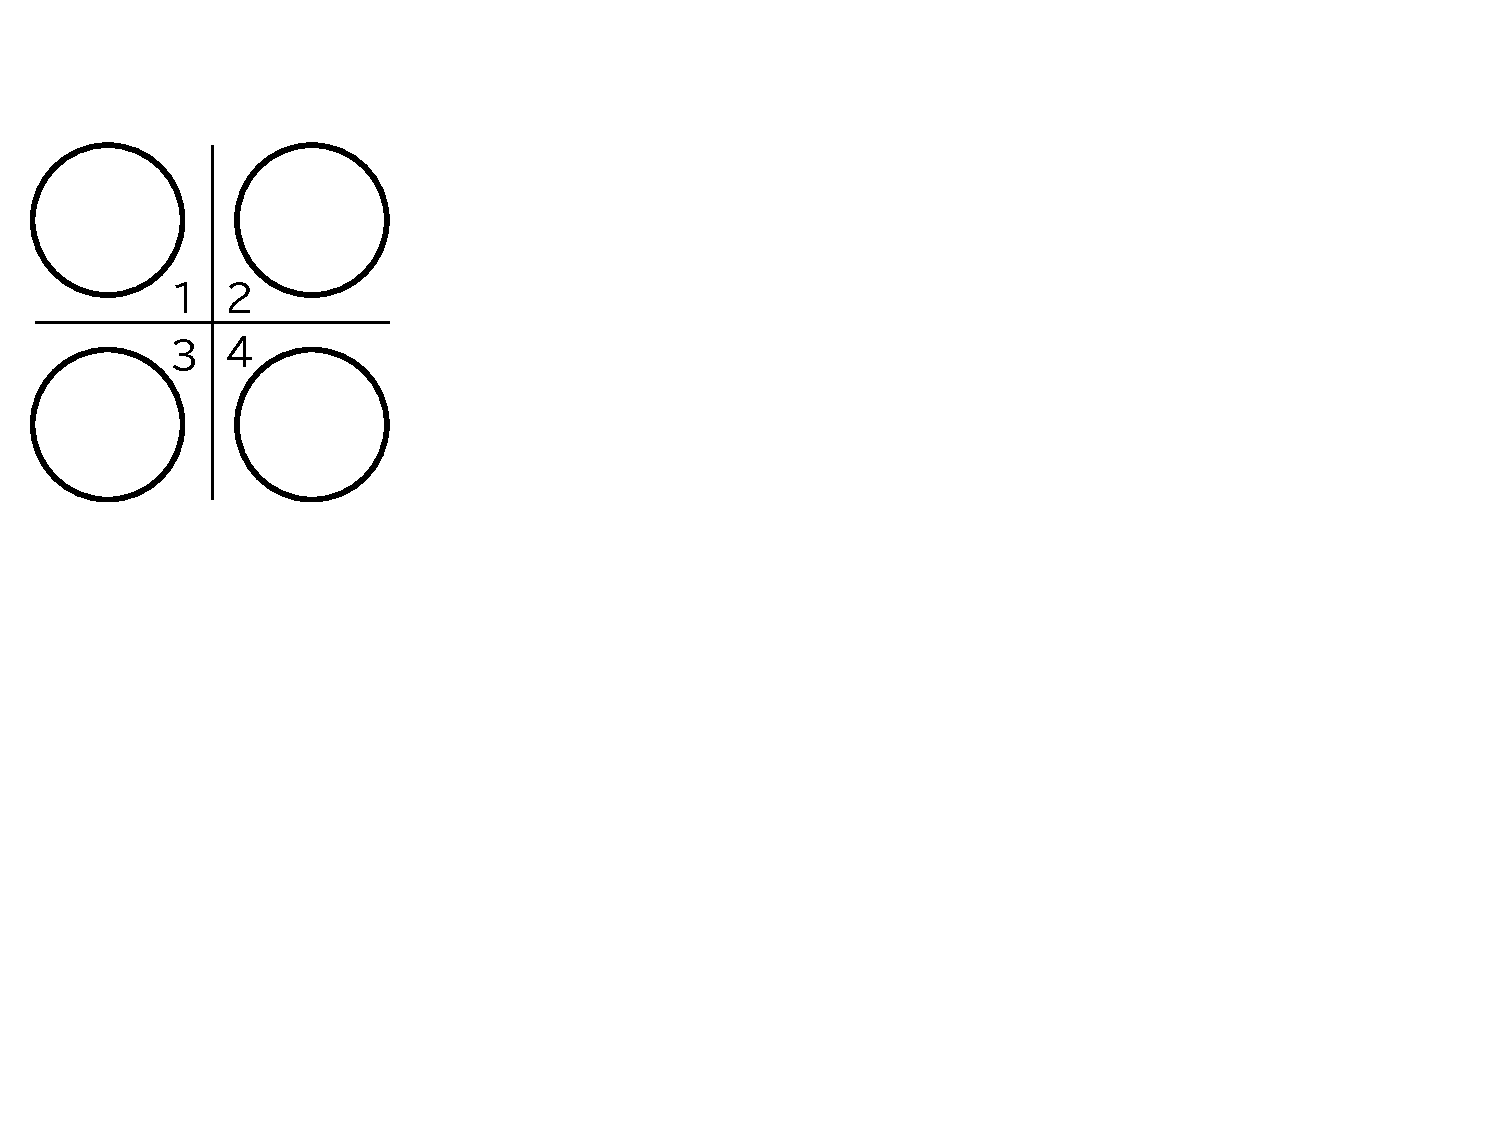
\includegraphics[width=3cm]{f1.pdf}\end{wrapfigure}